\documentclass[a4paper,english]{report}

\usepackage[latin1]{inputenc}
\usepackage[T1]{fontenc}
\usepackage{fourier}
\usepackage{babel,textcomp}
\usepackage[pdftex]{graphicx}
\usepackage{subfigure}
\usepackage{listings}
\usepackage{hyperref}
\usepackage{varioref}
\usepackage{cite}
\usepackage[color]{uiosloforside}
\usepackage{tikz}
\usetikzlibrary{shapes,arrows}

\setlength\topmargin{0in}
\setlength\headheight{0in}
\setlength\headsep{0in}
\setlength\textheight{8.7in}
\setlength\textwidth{6.5in}
\setlength\oddsidemargin{0in}
\setlength\evensidemargin{0in}
\setlength\parindent{0.25in}
\setlength\parskip{0.15in}
\setlength\columnsep{0.25in}

\definecolor{dkgreen}{rgb}{0,0.6,0}
\definecolor{gray}{rgb}{0.5,0.5,0.5}
\definecolor{mauve}{rgb}{0.58,0,0.82}
\definecolor{matnat}{rgb}{0.004,0.47,0.44}

% "define" Scala
\lstdefinelanguage{scala}{
  morekeywords={abstract,case,catch,class,def,
    do,else,extends,false,final,finally,
    for,if,implicit,import,match,mixin,
    new,null,object,override,package,
    private,protected,requires,return,sealed,
    super,this,throw,trait,true,try,
    type,val,var,while,with,yield},
  otherkeywords={=>,<-,<\%,<:,>:,@}, % Removed \#, because of Ruby comments error
  sensitive=true,
  morecomment=[l]{//},
  morecomment=[n]{/*}{*/},
  morestring=[b]",
  morestring=[b]',
  morestring=[b]"""
}

\lstset{basicstyle=\footnotesize,
  numbers=none,
  numberstyle=\tiny\color{gray},
  keywordstyle=\color{blue},
  commentstyle=\color{dkgreen},
  stringstyle=\color{mauve},
  frame=single,
  showstringspaces=false,
  breaklines=true,
  breakatwhitespace=true,
  tabsize=3,
  language=scala
}

\hypersetup{pdfborder={0 0 0},colorlinks=true,linkcolor=blue,urlcolor=blue,citecolor=blue}

\newcommand{\matlab}{\textsc{Matlab}\textregistered}

\title{Embedding Efficient DSLs on the Java Virtual Machine}
\author{Eivind Barstad Waaler (\emph{eivindwa})}

\begin{document}
\uiosloforside[kind={Master thesis},boxcolor=matnat,textcolor=white]

\chapter*{Abstract}
\addcontentsline{toc}{chapter}{Abstract}

Scala is an increasingly popular programming language running on the
JVM (Java Virtual Machine). One of its pronounced goals is to simplify
the creation of DSLs (Domain-Specific Languages) with extensible
syntax and combination of Object-Oriented and Functional
Programming. This thesis examines these possibilities with regard to
performance. It is demonstrated how you can use Scala to create
efficient DSLs on the JVM, utilizing parallel and concurrent
mechanisms found in modern computers.

\tableofcontents

\listoftables

\listoffigures

\chapter*{Preface}
\addcontentsline{toc}{chapter}{Preface}

This is a master-thesis of 60 credits\footnote{Prescribed to one year
  of full time study} in the field of Informatics. It was written for
the Object-orientation, Modelling, and Languages research
group\cite{oms} at the Department of Informatics, Faculty of
Mathematics and Natural Sciences, University of Oslo.

I would like to dedicate this work to the memory of my grandfather
Bjarne A. Waaler. His constant search for knowledge and truth has been
an enormous inspiration. I am proud to make a contribution to the same
university where he spent so many of his years working.

I would also like to thank my wonderful wife Anniken for the support
and understanding she has shown during this process. Her polite
reminders when my geeky interests go out of bounds are invaluable.

At last, but not least, I would like to thank my supervisor Professor
Birger M�ller-Pedersen at the Department of Informatics, UiO. His
unique experience from projects such as the \textsc{beta} programming
language \cite{beta} and the \textsc{swat} project\cite{swat} has
proven extremely valuable for me. Through many good discussions at his
office I've learned much about current and historic programming
language concepts. His enthusiasm has motivated me from beginning to
end.

\begin{flushright}
\textsc{Eivind Barstad Waaler}\\
Oslo, Norway\\
May 2010
\end{flushright}

\chapter{Introduction}
\label{sec:introduction}

The goal of this chapter is to describe the problem at hand as
detailed as possible. It has taken me a long time to clarify and
understand the problem, and as such I think it is justified to spend
quite a lot of time and space describing the background and why I
think it is important. The last part of the chapter describes the
methods used, and explains the structure of the rest of the document.

\section{Problem Formulation}
\label{sec:problemformulation}

\textit{Evaluate some major alternative programming languages on the
  Java Virtual Machine with regards to embedding Domain Specific
  Languages. Identify important aspects when working with embedded
  Domain Specific Languages and show what programming languages are
  suited and how they solve the problems.}

\section{Domain Specific Languages}
\label{sec:dsls}

\textit{``Domain-specific languages (DSLs) are languages tailored to a
  specific application domain. They offer substantial gains in
  expressiveness and ease of use compared with general-purpose
  programming languages.''}\cite{mer05}

DSLs are often categorized in two major types; external and embedded
(or internal) DSLs. An external DSL is a separate programming language
with custom syntax and a full parser, like SQL (domain of database
queries), CSS (domain of HTML styles) and XML (domain of data
exchange). An embedded DSL on the other hand, is created in a host
language. Various capabilities in the host language are exploited to
create interfaces that look and behave almost like a particular
programming language.

In this thesis I have identified different requirements of embedded
DLSs running on the Java Virtual Machine (JVM), and looked at how
various programming languages (described in section
\vref{sec:programminglanguages}) solve these aspects. As described in
the next section the exact definition of an embedded DLS is hard to
find, and as such this thesis is just as much a study of different
programming languages and what capabilities they provide.

\subsection{Embedded DSL or just Advanced Library Design?}
\label{sec:embeddeddsl}

It is difficult to draw a precise line between an embedded DSL and a
regular library. If you have a library specialized to solve problems
in a given domain, is that enough to call it an embedded DSL? How much
``special syntax'' do you need to include in the library to make it a
DSL? What kind of syntax qualifies for DSL use? Answering questions
like these is difficult, and in my opinion not contributing to a
fruitful discussion. I have tried to turn my focus toward interesting
capabilities different languages have, and the problems they solve. As
such some of the examples I will be using might not qualify as
embedded DLSs, but merely as libraries/interfaces with untraditional,
or in other ways interesting, use of the host language.

Martin Fowler and Eric Evans have defined the name ``fluent
interface''\cite{fow05} to describe interfaces which provide a more
readable and ``flowing'' syntax. Many of the examples given of fluent
interfaces are small libraries solving tasks in a specific domain, and
as such are also good examples of embedded DSLs. Eric Evans has also
written a book\cite{eva04} and held a number of talks on the subject
of Domain-Driven Design (DDD), a way of thinking and prioritizing when
working with software projects that deal with complicated domains. DDD
hardly covers the subject of embedding DSLs, but I feel that a lot of
the DSL design is focused on understanding and expressing a particular
domain and as such has a lot in common with the thoughts behind DDD.

The reason I include the section with this discussion is to briefly
try to demonstrate that the area of embedded DSLs is a complex and
maybe not precicely defined. The activity of building an embedded DSL
is tightly connected to the understanding of the domain at hand, and
the capabilities required from the host language will vary strongly
with that understanding. The next section gives a list of such
requirements.

\subsection{Requirements of an Embedded DSL}
\label{sec:requirements}

The following lists the different requirements/capabilities that might
be important when building embedded DSLs. The list provides a
foundation for structuring the rest of this report:

\begin{itemize}
\item Conciseness/``fluency'' -- What capabilities does the different
  languages provide in building fluent interfaces?
\item Use/reuse -- How can the DSL be used? How can several DSLs be
  combined?
\item Tool support -- What is the level of tool support provided for
  the DSL?
\item Error handling/reporting -- How are errors and exceptional
  situations handled in the different languages?
\item Performance -- How does the different languages facilitate
  building DSLs with high requirement regarding
  throughput/performance?
\end{itemize}

\section{JVM Programming Languages}
\label{sec:programminglanguages}

The goal platform of this thesis is the Java Virtual Machine
(JVM). The reason for this is that the enormous popularity of the Java
programming language has made the JVM one of the most widespread
multi-language platforms in the world. At the same time the Java
language itself is getting old, and many other languages have been
written (or ported) for the JVM. So this thesis looks at how some of
these languages provide various capabilities when building embedded
DSLs. I have tried to look at languages that differ in many
categories, as typing, paradigm or execution model. The languages I
have studied are described and categorized in the next sections.

\subsection{Categories of Languages}

I have chosen to categorize the languages in three different ways:

\begin{itemize}
\item Typing (static/dynamic) -- Static typing means that the majority
  of its type checking is enforced during compile-time, as opposed to
  run-time. The opposite is dynamic typing which performs most of its
  type checking during run-time.
\item Paradigm (OO/FP) -- There are many different programming
  paradigms. I have looked at object-oriented and functional
  programming languages. One of the languages (Scala) is a
  multi-paradigm language, combining object-orientation and functional
  programming techniques.
\item Execution (compiled/interpreted) -- On the JVM an interesting
  way to categorize programming languages is wether they are compiled
  to byte-code and run directly on the virtual machine, or if the
  language is interpreted and run by some extra layer on top of the
  JVM.
\end{itemize}

\subsection{Java}

\subsection{Ruby/JRuby}

\subsection{Groovy}

\subsection{Clojure}

\subsection{Scala}

\textit{``Scala is a general purpose programming language designed to
  express common programming patterns in a concise, elegant, and
  type-safe way. It smoothly integrates features of object-oriented
  and functional languages, enabling Java and other programmers to be
  more productive. Code sizes are typically reduced by a factor of two
  to three when compared to an equivalent Java
  application''.}\cite{scala}

Scala is a relatively new language (first version released
2003\cite{scala}) providing exciting programming capabilities on the
Java Virtual Machine (JVM). The main reason for chosing Scala in this
thesis is the combination of powerful programming structures (both
object-oriented and functional) with the cross-platform and wide
adoption of the JVM. Code written in Scala can be run on any JVM
version 1.5 or newer, and can utilize any library written in Java. It
can thus be seen as a <<best of both worlds>> language.

The following sections describe properties of Scala that might make it
suited for building <<high performance DLSs>> on the JVM. For more
detailed information about Scala please refer
to\cite{ode08},\cite{scala} or\cite{scalatour}.

\subsubsection{Scala and Java}
\label{sec:scalajava}

Scala code (.scala files) compiles to Java bytecode (.class files)
through a special compiler (\texttt{scalac}). The bytecode can then be
run on the JVM as if it was created from Java source (.java files). In
adition Scala provides a number of library classes that need to be
included as a jar file. This relationship between Scala and Java is
illustrated in figure \vref{fig:scalajava}.

\begin{figure}
  \begin{center}
  \tikzstyle{block} = [rectangle, draw, fill=blue!20, text width=5em, text centered, rounded corners, minimum height=4em]
  \tikzstyle{line} = [draw, -latex']
  \tikzstyle{cloud} = [draw, ellipse,fill=red!20, text width=5em, text centered, node distance=2.5cm, minimum height=2em]
  \begin{tikzpicture}[node distance = 2cm, auto]
    % Place nodes
    \node [cloud] (class) {Java Bytecode (.class)};
    \node [block, left of=class, above of=class] (scalacompile) {Scala Compile (scalac)};
    \node [cloud, left of=scalacompile] (scala) {Scala Source (.scala)};
    \node [block, right of=class, above of=class] (javacompile) {Java Compile (javac)};
    \node [cloud, right of=javacompile] (java) {Java Source (.java)};
    \node [block, below of=class] (jvm) {Java Virtual Machine};
    \node [block, below of=scala] (scalalib) {Scala API (.jar)};
    % Draw edges
    \path [line] (scalacompile) -- (class);
    \path [line] (javacompile) -- (class);
    \path [line] (class) -- (jvm);
    \path [line] (scala) -- (scalacompile);
    \path [line] (java) -- (javacompile);
    \path [dotted, line] (scalalib) -- (jvm);
  \end{tikzpicture}
  \end{center}
  \caption{Visual representation of the relationship between Scala and
    Java.\label{fig:scalajava}}
\end{figure}

The tight relationship with Java has a number of advantages when using
Scala:

\begin{itemize}
\item Cross-platform distribution -- Code written in Scala can be run
  on any platform supporting JVM 1.5 or newer.
\item Stability and standards -- The JVM is a stable platform with
  good support for internationalization (Unicode support ++) and
  localization (supports local languages and standards).
\item Access to libraries -- The JVM has a wide range of libraries
  available, many being Open Source.
\item High performance -- The JVM has been proven to be a high
  performant Virtual Machine, with a large number of tuning
  possibilities.
\end{itemize}

There are also disadvantages with such a tight coupling to the JVM:

\begin{itemize}
\item Limitations in bytecode -- Scala, being a functional language,
  would benefit from features not present in the current version of
  the JVM. Most notably is the (lack of) support for full tail call
  optimization, which would improve performance of recursive
  functions.
\item Generics implemented with erasure -- Scala uses an erasure
  scheme to implement generics, to be 100\% compatible with
  Java. However, the implementation of the Scala compiler
  (\texttt{scalac}) has some advanced solution to many of the problems
  Java has regarding erasure\cite{emi06}.
\end{itemize}

\section{Method}
\label{sec:method}

This section describes the research methods applied in this
thesis. In\cite{dyb08} the concept ``Evidence-Based Software
Engineering'' (EBSE) is introduced. Although this article is mainly
targeted towards practicioners looking to support decision-making I
feel that it gives a good foundation for evaluating research methods
related to Software Engineering. The main steps of EBSE are as
follows:

\begin{enumerate}
\item Convert a relevant problem or need for information into an
  answerable question.
\item Search the literature for the best available evidence to answer
  the question.
\item Critically appraise the evidence for its validity, impact, and
  applicability.
\item Integrate the appraised evidence with practical experience and
  the client's values and circumstances to make decisions about
  practice.
\item Evaluate performance in comparison with previous performance and
  seek ways to improve it.
\end{enumerate}

With this list as basis I ended up with the following steps for this
thesis:

\begin{enumerate}
\item Create answerable questions -- Make sure the questions to
  research are sound and possible to answer.
\item Search existing literature -- Find literature to provide direct
  answers to the questions, or to support assumptions needed to
  sustain experiments.
\item Critically appraise the literature evidence -- Make sure the
  chosen literature actually provide valid evidence for its claims.
\item Conduct experiments -- The major part of the thesis work is of
  course related to the experiments conducted. The first three steps
  are important to make sure the experiments are based on sound
  evidence and former knowledge.
\item Critical evaluation -- The experiments and results found must be
  carefully evaluated. By being critical to my own results I hope to
  improve the overall quality of the thesis deliverance.
\end{enumerate}

\subsection{Report Structure}

\chapter{DSL Syntax}
\label{sec:dslsyntax}

The syntax of a language defines its surface form\cite{fri08}. It is
the set of rules that define the combinations of symbols that are
considered to be correctly structured programs in that language. So a
DSL is defined in terms of its syntax. For an embedded DSL its syntax
describes special ways to use the host language. This chapter
describes various programming language concepts that can be useful
when designing an embedded DSL. The final section concludes on some
major differences between various classes of host languages and what
these mean to the construction of embedded DSLs.

\section{Function Chaining/Nesting}

TODO: Rewrite to summarize fluent interfaces (Fowler + Evans). Example use\cite{fre06}.

One of the simplest ways to create a DSL-like syntax is to allow
chaining several function calls together. As an example consider the
following Java-code (from\cite{fow06}), where the construction of a
\texttt{HardDrive} object is shown with and without method chaining:

\begin{lstlisting}[language=java]
// Construct with setter methods
HardDrive hd = new HardDrive();
hd.setCapacity(150);
hd.setExternal(true);
hd.setSpeed(7200);

// Construct with method chaining
HardDrive hd = new HardDrive().capacity(150).external().speed(7200);
\end{lstlisting}

The chaining of methods can also be combined with method nesting,
grouping methods that belong together (also from\cite{fow06}):

\begin{lstlisting}[language=java]
computer(
  processor(
    cores(2),
    Processor.Type.i386
  ),
  disk(
    size(150)
  ),
  disk(
    size(75),
    speed(7200),
    Disk.Interface.SATA
  )
);
\end{lstlisting}

Function chaining is available in most programming languages. In
functional programming it is a fundamental concept, while in
object-oriented langauges more a design choice (as in the example
above). In object-oriented languages using function chaining is often
referred to as building \texttt{fluent interfaces}.

\section{Static Methods/Singleton Objects}

In object-oriented languages functions are nested inside classes. In
order to be able to call functions without instantiating objects we
have static methods, that are associated directly with the class
instance and not with objects created from the class. The following
example shows how to sort a list of strings in Java, using the static
method \texttt{sort} in the \texttt{Collections} class:

\begin{lstlisting}[language=java]
// Create a list of strings
List<String> names = ...

// Sort the list
Collections.sort(names);
\end{lstlisting}

A different approach to static methods is the singleton objects found
in Scala. Instead of having methods defined as static there is a
notion of a singleton object, as in the following example defining
sorting similar to the Java-example above:

\begin{lstlisting}
// Define ListSorter object
object ListSorter {
  def sort(list: List) { ... }
}

// Use object
var names = List("name1", "name2")
ListSorter.sort(names)
\end{lstlisting}

Static methods may play a central role in an embedded DSL, especially
combined with \texttt{Member Imports} (next section). They are
typically used for object creation through patterns like
\texttt{Factory method} and \texttt{Builder}, or other utility
operations like the sorting shown in the examples above.

\section{Member Imports}

Member imports is a very useful mechanism in object-oriented languages
for creating concise syntax, and thus in the embedding of DSLs. Using
static member import the Java sorting example from previous section
could have been written like this:

\begin{lstlisting}[language=java]
import static java.util.Collections.*; // Import all static members of the Collections class
...

// Create a list of strings
List<String> names = ...

// Sort the list
sort(names);
\end{lstlisting}

In Scala member imports are less restricted than in Java. They can be
used anywhere in the code (not just at the start of the file), and are
not restricted to static members.

\begin{lstlisting}
class Fruit(val name: String, val color: String) // Define class Fruit with two members

val apple = new Fruit("apple", "red") // Create apple as instance of Fruit

import apple._ // Import all members from object apple

println(name + " is " + color) // Access members 'name' and 'color' directly
\end{lstlisting}

\section{Method Names and Operator Notation}

When constructing an embedded DSL we like to make the syntax reflect
the actual domain as much as possible. Having flexible ways to name
and call methods can be a very useful property of a host language.

Scala has two features regarding method names and syntax that are
interesting with regards to DSL development\cite{dub06}:

\begin{itemize}
\item Arbitrary method names - Scala methods can have special
  characters as names. As such Scala has full support for operator
  overloading, as operators are just regular methods with special
  names. For example \texttt{+}, \texttt{!=} and \texttt{<=}.
\item Operator notation - Methods in Scala can be called without the
  dot and parentheses, as shown in the examples below.
\end{itemize}

\begin{lstlisting}
abstract class Matrix {
  // Method names can be operators
  def +(other: Matrix) = add(other)
  // Regular method name
  def add(other: Matrix): Matrix // Abstract method
}

// Usage example - regular notation
val m3 = m1.+(m2)
val m3 = m1.add(m2)
// Operator notation
val m3 = m1 + m2
val m3 = m1 add m2
\end{lstlisting}

In the dynamic language Ruby they have a similar mechanism as in
Scala. Here you are allowed to leave the parentheses surrounding the
parameter(s) out, but not the dot in front of the method name.

\begin{lstlisting}[language=Ruby]
name = "John"

# Method without parameters
name.empty?()
name.empty?

# Method with one parameter
name.include?("e")
name.include? "e"
\end{lstlisting}

\section{Special Syntax Constructs}

Many programming languages have special constructs that are made
specifically to enable the writing of concise statements. Typically
constructs that only offer a different syntax that will be replaced by
the compiler at early phases of compilation. The next sub-sections
describe some examples of such mechanisms.

\subsection{The ``magic'' \texttt{apply} Method}
\label{sec:applymethod}

Scala uses the \texttt{apply} method to let classes and object define
functionality that appears to be native in the language. You can leave
the method name out and simply write syntax that seems to pass
parameters directly to an object. In the following example the
\texttt{apply} method is used to index the \texttt{Matrix} class as if
it was a native feature:

\begin{lstlisting}
class Matrix[T] {
  def apply(row: Int, col: Int): T = ...
}
val intMatrix = ... // Matrix[Int]
// Get Int at position 2, 4
val intVal = intMatrix(2, 4) // Replaced by compiler: intMatrix.apply(2, 4)
\end{lstlisting}

\subsection{Query Syntax}

In C\# 3.0 a DSL called LINQ (Language Integrated Query) was
introduced. It is used to natively query data in the language. The
implementation of the DSL relies on a number of language features
(type inference, anonymous types, object initializer and lambda
expressions -- see sections below) in addition to the query syntax
itself.

\begin{lstlisting}[language={[Sharp]C}]
// Query syntax:
var results = 
  from c in SomeCollection
  let x = someValue * 2
  where c.SomeProperty < x
  select new {c.SomeProperty, c.OtherProperty};

// Resulting rewritten syntax:
var results =
  SomeCollection.Where(
    c => c.SomeProperty < (SomeValue * 2)
  ).Select( c => new {c.SomeProperty, c.OtherProperty} );
\end{lstlisting}

In Scala we have \texttt{for comprehensions} that can be viewed as a
query syntax much like that of LINQ. Complex expressions using the
mechanism will be rewritten to a combination of \texttt{filter},
\texttt{flatMap} and \texttt{map}:

\begin{lstlisting}
// "Query syntax" - for comprehension:
val results = for {
  name <- listOfNames
  if (name startsWith "E")
} yield { name toUpperCase }

// Resulting rewritten syntax:
val results = listOfNames.filter(_ startsWith "E").map(_ toUpperCase)
\end{lstlisting}

Daniel Spiewak has written a paper investigating the possibility to
extend the for comprehensions in Scala to support LINQ-style database
queries\cite{spi09}. Both mechanisms rely on monadic behaviour
(concept from functional programming), where complex statements can be
constructed by combining a set of basic functions (as shown in the
examples above).

\section{Type Inference}

With type inference the compiler will figure out the type of a value
or function, so there is no need to explicitly specify it. This is
useful when writing embedded DSLs, to give a less verbose and more
concise syntax. Some examples were given in the previous section about
query syntax.

The Scala compiler will try to infer the types used. So if the type is
obvious there is no need to specify it:

\begin{lstlisting}
val i = 42 // Type Int is infered
val d = i + 2.1 // Type Double is infered
val iBy2 = (i: Int) => i * 2 // Return value Int is infered from int parameter
val dBy2 = (i: Double) => i * 2 // Return value Double is infered from int parameter
\end{lstlisting}

\section{Implicit Type Conversion}
\label{sec:implicit_type_conversion}

Implicit type conversions are used to allow the compiler to
automatically convert one type to another where possible. From a DSL
syntax perspective this is used to "add" new methods to existing
types. This can be built-in types or user-defined types. In the
following Scala example an implicit conversion is used to convert from
\texttt{Int} to \texttt{MyInt}, and thus allowing the
\texttt{doubleIt} method to be called directly on the integer value:

\begin{lstlisting}
// Wrapper class for int
class MyInt(val i: Int) {
  def doubleIt = i * 2 // Method
}
// Implicit conversion
implicit def fromInt(i: Int) = new MyInt(i)
// Convert Int to MyInt and call method
val ten = 5.doubleIt
\end{lstlisting}

In dynamic languages a mechanism that can give much the same results
is Monkey Patching described in section
\vref{sec:monkey_patching}. Implicit conversions are also very useful
when combining DSLs. This is described in
section\vref{sec:combining_dsls}.

\section{Lambda Expressions/Anonymous Functions}

Anonymous functions, or lambda expressions, can be used as parameters
for higher-order function (functions using functions as parameters or
return values). This is maybe not directly relevant for embedded DSL
syntax, but is an important building block in query syntax (shown in a
previous section). For example in the Scala for comprehensions and the
LINQ statements shown in an earlier section, anonymous functions play a
role in allowing filtering (if-statements).

\section{Anonymous Types}

Anonymous types allow the construction of types without a name, based
on fields. Combined with type inference this is a central feature in
the implementation of LINQ (as described in an earlier section).

Scala also supports anonymous types. An example of using anonymous
types together with type inference:

\begin{lstlisting}
val person = new { val name = "John"; val age = 26 }

println(person.name + " is " + person.age + " years old..")
\end{lstlisting}

In LINQ this is used to allow selection of fields from a database or
other data structure:

\begin{lstlisting}[language={[Sharp]C}]
var results = 
  ... // Some query
  select new {c.SomeProperty, c.OtherProperty};
\end{lstlisting}

\section{Object Initializer}

Object initializers provide the ability to give values to an object
while instantiating it. In C\# this can look like the following, and
is also used to select objects of given class instead of anonymous
types from LINQ:

\begin{lstlisting}[language={[Sharp]C}]
val results =
  ... // Some query
  select new Person { Name = c.SomeProperty, Age = c.OtherProperty }
\end{lstlisting}

Scala also support object initializers, as in the following example:

\begin{lstlisting}
class Person {
  var name = ""
  var age = 0
}

val person = new Person { name = "John"; age = 26 }
\end{lstlisting}

\section{Metaprogramming}

Metaprogramming is the writing of computer programs that write or
manipulate other programs (or themselves) as their data, or that do
part of the work at compile time that would otherwise be done at
runtime. In terms of embedded DSL creation, metaprogramming is used in
some dynamically typed programming languages to create interesting
possibilities.

A typical example of a DSL utilizing metaprogramming is the Rails
framework and the \texttt{ActiveRecord} class. Here metaprogramming is
used to specify relationships between the classes \texttt{Team} and
\texttt{Player}:

\begin{lstlisting}[language=Ruby]
class Team < ActiveRecord::Base
  has_many :players
end

class Player < ActiveRecord::Base
  belongs_to :team
end

# Now a player will have a 'team' method returning the team
player.team

# And a team will have a 'players' method returning a collection of players
team.players.each { |team| ... }
\end{lstlisting}

\section{Open Classes/Monkey Patching}
\label{sec:monkey_patching}

A monkey patch is a way to extend or modify the runtime code of
dynamic languages without altering the original source code. In DSL
creation this can be used in much the same way as implicit
conversions, by adding new functionality to built-in or other
types. In the following code we re-implement with open classes/monkey
patching the same example shown earlier with implicit type
conversions:

\begin{lstlisting}[language=Ruby]
class Integer
  def doubleIt
    self * 2
  end
end

ten = 5.doubleIt
\end{lstlisting}

\section{Dynamic Dispatch -- Method Missing}

Dynamic programming languages use dynamic dispatch to determine what
code to run when a message is received. This means that errors related
to missing methods are postponed until runtime. Some languages provide
interesting ways to handle these errors, that can be utilized in DSL
creation.

In Ruby there is a notion of custom dispatch behaviour that can be
controlled by the programmer. The base class, that all other classes
extend from, has a \texttt{method\_missing} method that is called by
the dispatcher as a last resort when no other method is found to
respond to a message. The default behaviour is to throw a
\texttt{NoMethodError}, but this can be overridden by extending
classes.

To see how this can be used in a DSL we can look at a simplified
version of the \texttt{ActiveRecord} class from the \texttt{Rails}
framework. It maps objects to database tables and allows dynamic
querying through the DSL syntax:

\begin{lstlisting}[language=Ruby]
class ActiveRecord
  # ...
  def self.method_missing(method_id, *arguments)
    if match = /find_(all_by|by)_([_a-zA-Z]\w*)/.match(method_id.to_s)
      # ... extract column names from match, generate and run SQL expression + map and return results
    end
  end
end

# Define class 'Person' as extension of 'ActiveRecord'
class Person < ActiveRecord::Base
end

# Query the database for person with given username
person = Person.find_by_username "eivindw"
\end{lstlisting}

\section{Conclusion}

Modern statically typed languages like Scala offer some very powerful
features for building embedded DSLs, combining concepts from
object-oriented and functional programming languages. Advanced type
systems offering type interference, implicit conversions and anonymous
types provide powerful mechanisms when constructing DSLs, removing
much of the verbosity often associated with statically typed
languages.

When comparing various classes of programming languages the biggest
difference with regards to DSL syntax seems to be that between static
and dynamic languages. Even with feature rich static programming
languages like Scala there are a series of concepts from dynamic
languages which does not have a natural counterpart in the statically
typed domain. Most notebly are the powerful metaprogramming features
found in many dynamic languages and the dynamic dispatch mechanism
allowing custom handling of missing methods.

\chapter{DSL Composition}

\section{Modular DSL Composition}

\subsection{Traits - Polymorphic Abilities}

Scala has support for virtual types (abstract type members) and
familiy polymorphism\cite{ode03}, mixin composition\cite{ode05} and
higher-order genericity\cite{moo08}. These are all powerful features
that support polymorphic embedding of DSLs\cite{hof08}.

This allows building DSLs that can have several different
interpretations as reusable components. It can also be used to
effectively combine different DSLs into new ones. The paper
``Polymorphic Embedding of DSLs''\cite{hof08} describes this in detail
with examples.

A use of traits can be to split functionality in several traits and
create classes/objects with only the methods that we need. In the
following example the \texttt{Matrix} class does not have any methods,
but instances of the class can be mixed in with traits containing
various methods:

\begin{lstlisting}
class Matrix {} // No methods

trait AvgMtx { this: Matrix =>
  def avg(): Matrix = { ... }
}

trait MorphMtx { this: Matrix =>
  def erode(): Matrix = { ... }
  def dilate(): Matrix = { ... }
}

// Matrix with only avg() method
val m1 = new Matrix with AvgMtx
// Matrix with erode() and dilate() methods
val m2 = new Matrix with MorphMtx
// Matrix with "all" methods
val m3 = new Matrix with AvgMtx with MorphMtx
\end{lstlisting}

\section{Combining DSLs}
\label{sec:combining_dsls}

\subsection{Implicit Conversion}

Implicit type conversions where described in
section\vref{sec:implicit_type_conversion}, in terms of DSL syntax. In
this section we will look at how implicits can be used to combine
functionality from two different DSLs.

\begin{lstlisting}
val ds = DataSet(1, 2, 3, 4, 5, 6, 7, 8, 9)

assert(5.0 === ds.average)
assert(1 === ds.min)
assert(9 === ds.max)
\end{lstlisting}

\begin{lstlisting}
val words = Array("eivind", "test", "oslo", "bekk", "scala", "elephant", "cat")

implicit def str2DS(str: Array[String]) = {
  DataSet(str.map(_.length): _*)
}

assert(5 === words.average.round)
assert(3 === words.min)
assert(8 === words.max)
\end{lstlisting}

\begin{lstlisting}
val img = Image(Matrix(3, List(
  9, 8, 7,
  6, 5, 6,
  7, 8, 9)))

implicit def img2DS(img: GrayScaleImage) = {
  DataSet(img.data.toArray: _*)
}

assert(7 === img.average.round)
assert(5 === img.min)
assert(9 === img.max)
\end{lstlisting}

\chapter{Advanced DSL Techniques}

\section{Removing from Host Language -- Pruning}

\section{Extending Host Language}

\chapter{Using the DSL}

\section{Scripting}

\section{API/Library}

\section{Interactive Console -- Interpreter}

\section{Embedded Interpreter}

\section{Tool Support}

\chapter{DSL Performance}

\section{Host Language -- Dynamic vs. Static Typing}

\section{Code Efficiency}

\section{Multithreading -- Parallel Computing}

\section{Distributed DSL}

\section{Secondary Processors -- GPU}

\chapter{Examples}

\section{DSL for Image Processing}

\subsection{Description}

Image Processing is an area involving series of computationally heavy
operations performed on images. Many practicioners in the area have
more mathematical than computer science oriented background. This
leads to the need for DSLs where complicated and computationally heavy
operations can be performed with a simple and straightforward syntax.

A major actor in the art of Image Processing is the product \matlab
from the company MathWorks\texttrademark. They provide the user with a
DSL for doing advanced Image Processing operations. I have tried to
create a similar DSL (with limited functionality) in Scala.

As an example consider the operation of blurring an image using an
average filter mask show in figures \vref{fig:eximg} and
\vref{fig:exavg}. This is a basic operation, but serves good as an
example of using the DSLs.

The \matlab{} code to perform the operation could
typically look like this:
\begin{lstlisting}[language=matlab]
img = imread('cell.jpg');
% 3x3 neighborhood default
imgAvg = medfilt2(img);
imwrite(imgAvg, 'cell_avg.jpg');
\end{lstlisting}

My goal is to create a Scala DSL to achieve the same result. A
suggested Scala-solution to the problem will look something like this:

\begin{lstlisting}
// Imports...
val img = loadImageCP("/cell.jpg")
val se = StrEl(Square, 3)
val imgAvg = img.avg(se)
saveImage(imgAvg, "/cell_avg.jpg")
\end{lstlisting}

\begin{figure}
  \subfigure[Original]{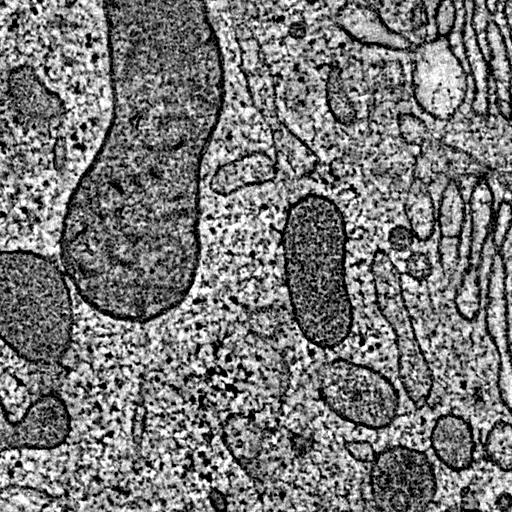
\includegraphics[width=0.49\textwidth]{images/cell}}
  \hfill
  \subfigure[Blurred]{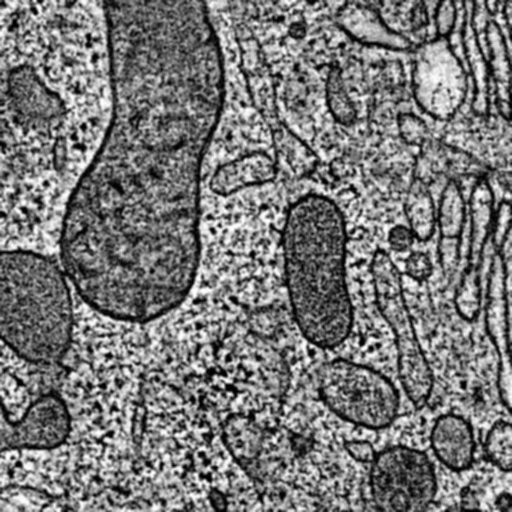
\includegraphics[width=0.49\textwidth]{images/cell_avg}}
  \caption{Example image before and after blurring with average
    filter.\label{fig:eximg}}
\end{figure}

\begin{figure}
  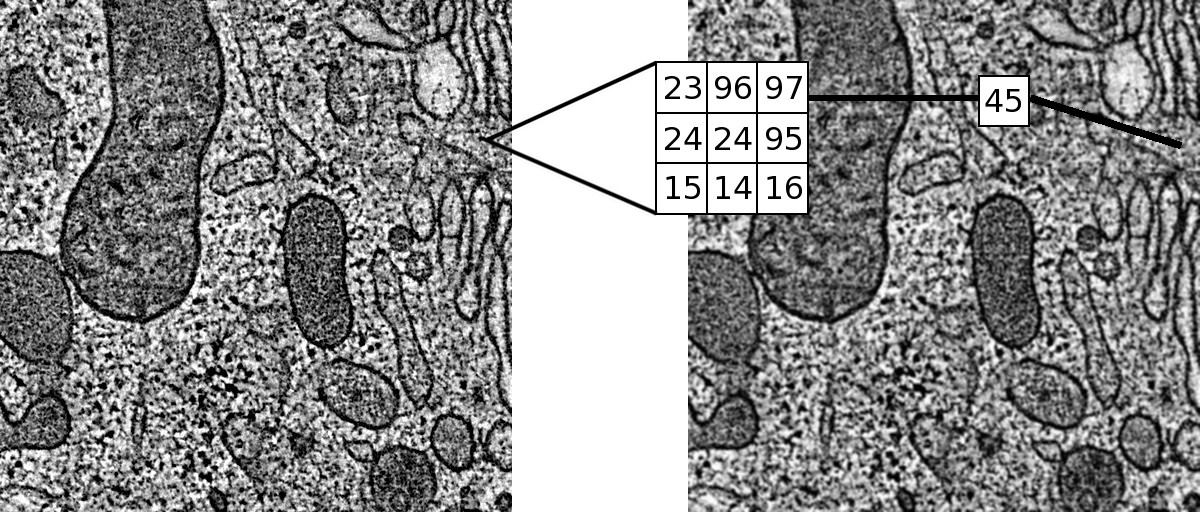
\includegraphics[width=1.0\textwidth]{images/avg_process}
  \caption{Visualising the process of blurring an image using average
    filtering with a 3x3 neighbourhood.\label{fig:exavg}}
\end{figure}

The rest of this section describes how I implemented this, and what
the results where with regards to the performance (how efficient the
implementation is).

\subsection{Syntax}

The methods to load and save the image, as well as the \texttt{Square}
definition of structuring element, are all member functions in classes
\texttt{SImageIO} and \texttt{StrElType}. These can be imported with
the \texttt{.\_} notation in Scala, and are then available directly:

\begin{lstlisting}
import io.SImageIO._
import structs.StrElType._

// SImageIO.loadImageCP("/cell.jpg")
val img = loadImageCP("/cell.jpg")
...
saveImage(imgAvg, "/cell_avg.jpg")

// StrElType.Square
val se = StrEl(Square, 3)
\end{lstlisting}

To create the structuring element, the \texttt{StrEl} trait has a
<<companion object>> with an \texttt{apply} method (described in
section \vref{sec:applymethod}. This gives a very compact syntax,
combined with the import of the available structuring element types as
shown above:

\begin{lstlisting}
object StrEl {
  import StrElType._
  def apply(t: StrElType, num: Int) = Array2DStrEl(t, num)
}

val se = StrEl(Square, 3)
\end{lstlisting}

Using traits, we are able to compose image objects with the operations
we want. The operations are implemented in separate traits which are
mixed in with the image on creation. This is using self-type
annotations to specify that the trait can only be mixed in with
classes of type \texttt{GrayScaleImage}:

\begin{lstlisting}
trait Standard { this: GrayScaleImage =>
  def avg(se: StrEl[Int]) = { ... }
}

object Image {
  import operations.{Morphology, Standard}

  def apply(d: Matrix[Int]) = {
    new GrayScaleImage(d) with Standard with Morphology
  }
}

val imgAvg = img.avg(se)

// Equivalent - operator notation
val imgAvg = img avg se
\end{lstlisting}

\subsection{Parallel Processing}

With images larger than a certain size, the operations performed in
the image analysis are bound to be heavy in terms of the number of
computations that need to be executed. This opens up a demand for
exploiting the capabilities found in modern computers with regard to
parallelization and concurrency. In the following sections we look at
different mechanisms available from the Scala language to achieve
better performance through utilization of the hardware resources
available in the computer. The first two sections discuss mechanisms
for concurrent programming on a multi-core/-processor environment,
while the third section discuss a mechanism for parallelization using
the GPU (Graphics Processing Unit).

\subsubsection{Actors API}
\label{sec:actors}

The primary concurrency construct in Scala is actors. Actors are
basically concurrent processes that communicate by exchanging
messages\cite{hal06}. My first attempt at making the Image Processing
DSL parallel was by making a generic executor using the Actors
API. The result, with an example of simple usage, is shown in figure
\vref{fig:actorexecutor}. Isolated parts of the processing can be
split into separate functions that are distributed over a set of
executors. So my example with a String operation is easily extended to
Image Processing or any other domain that can be split into several
parallel functions.

The main issue with this approach is that we need to wait for the
result to be ready. This is of course not a big problem, but the next
section describes another technique that is better suited for parallel
computing.

\begin{figure}
  \begin{lstlisting}
import actors.Actor
import actors.Actor._

// Message contains data and transformation function
case class ExecMsg[T <: Any](data: T, op: T => T)

// Executor executes function and exits
class Executor extends Actor {
  def hasResult = result != None

  def getResult = result

  private var result: Option[Any] = None

  def act {
    while(true) {
      receive {
        case ExecMsg(d, op) => result = Some(op(d)); exit
      }
    }
  }
}

// Example usage - convert "scala" to upper case in separate thread
val exec = new Executor
exec.start // Start running - ready to receive messages
exec ! ExecMsg("scala", (s: String) => s.toUpperCase) // Send data and function
while(!exec.hasResult) {} // Busy waiting..
println("Result: " + exec.getResult.get) // Prints "SCALA"
  \end{lstlisting}
  \caption{A generic \texttt{Executor} based on the Scala Actors
    API.\label{fig:actorexecutor}}
\end{figure}

\subsubsection{Futures API}
\label{sec:futures}

Actors may communicate using futures where requests are handled
asynchronously, but return a representation (the future) that allows
to await the reply. This is better suited for the parallel processing
we are trying to achieve. An example similar to the pure actor example
in the previous section using futures is shown in figure
\vref{fig:futureex}.

\begin{figure}
  \begin{lstlisting}
import actors.Futures._

// Define function - could also be done directly in the future-block below
val func = (s: String) => s.toUpperCase

// Create future running the function with the String argument
val fut = future { func("scala" }

// Wait for and return the result
println("Result: " + fut())
  \end{lstlisting}
  \caption{An example using \texttt{Futures} to execute a function in
    a separate thread.\label{fig:futureex}}
\end{figure}

Futures also support waiting for an array of functions to
complete. This is the mechanism used in the Image Processing DSL. See
figure \vref{fig:futureipex} for a complete example of how futures are
used to run several operation in parallel and merge the results once
all futures have finished running. The \texttt{Splittable} identifier
is simply a trait specifying \texttt{split} and \texttt{merge} methods
that need to be implemented by users of the \texttt{parallel}
function. Notice how the futures are yielded to a sequence directly
from the for comprehension and awaited completion using the
\texttt{awaitAll} function.

\begin{figure}
  \begin{lstlisting}
import actors.Futures._

object Operations {

  def parallel[T](obj: Splittable[T], op: (T) => Splittable[T]): Splittable[T] = {
    obj.split match {
      case Array(region) => op(region)
      case regions: Array[T] => {
        val futures = for(region <- regions) yield future {
          op(region)
        }
        val results = awaitAll(5000, futures: _*)
        val parts = for(result <- results) yield result.get.asInstanceOf[Splittable[T]]
        parts.reduceLeft(_ merge _)
      }
    }
  }
}

// Example usage - double values in the list in separate threads
case class MyList(val list: List[Int]) extends Splittable[Int] {
  def split = list.toArray
  
  def merge(other: Splittable[Int]): Splittable[Int] = (this, other) match {
    case (t: MyList, o: MyList) => new MyList(t.list ::: o.list)
  }
}

val splitList = MyList(List(2, 5, 7, 1))

val doubledList = parallel (
  splitList,
  (i: Int) => {
    Thread.sleep(100) // Slow things down a little
    new MyList(List(i * 2))
  }
).asInstanceOf[MyList]
  \end{lstlisting}
  \caption{A general parallel mechanism based on
    futures.\label{fig:futureipex}}
\end{figure}

\subsubsection{OpenCL with ScalaCL}
\label{sec:opencl}

Recent years manufacturers of graphics cards and GPUs (Graphics
Processing Unit) have made libraries available to run general code
(not just graphics processing) on their hardware. This is typically
hardware optimized for matrices and image processing, so it should be
very interesting to utilize this possibility to speed up the
operations in a Image Processing library.

OpenCL\texttrademark\cite{opencl} is an open standard for parallel
programming that utilizes the power of the GPU to perform
calculations. OpenCL is being created by the Khronos Group with the
participation of many industry-leading companies and institutions. A
Scala API exists which enables Scala programs to make use of the
possibilities offered by OpenCL -- ScalaCL\cite{scalacl}.

A simple example using ScalaCL to add two arrays of integers is shown
in figure \vref{fig:scalacl}.

\begin{figure}
  \begin{lstlisting}
import scalacl.{Dim, Program}
import scalacl.ScalaCL._

class SeOpOCL(i: Dim) extends Program(i) {
  val iarr = IntsVar
  val iarr2 = IntsVar
  
  var output = IntsVar
  
  content = output := iarr + iarr2
}

val arr1 = Array(1, 2, 3, 4, 5)
val arr2 = Array(5, 4, 3, 2, 1)

val prog = new SeOpOCL(new Dim(arr1.size))

prog.iarr.write(arr1)
prog.iarr2.write(arr2)

prog !

println("First: " + prog.output.get(0)) // Print 6
  \end{lstlisting}
  \caption{Add two arrays of integers using
    ScalaCL\label{fig:scalacl}}
\end{figure}

\subsection{Efficient Implementation Tips}
\label{sec:effimpl}

When performing the same operation a large number of times, as is the
case with many algorithms for Image Processing, there are various
implementation related things that need to be considered. In this
section I summarize the lessons learned with regards to tuning the
code for maximum performance.

\subsubsection{Choice of data structures}
\label{sec:datastructures}

The underlying data structure for images and Image Processing is the
matrix. Since Scala does not include an efficient implementation of
matrix I ended up testing a few different variants:

\begin{itemize}
\item \textbf{List of Lists} -- A very logical implementation of
  matrix is by using Scala \texttt{Lists}. The idea for this
  implementation was inspired by a blog post by Jonathan
  Merritt\cite{mer08}. A simple example of using a list of lists is
  shown in figure \vref{fig:listoflist}. However, this implementation
  proves to be very slow in specific element access and iteration.
\item \textbf{2D Array} -- In Scala an \texttt{Array} will usually be
  faster than \texttt{List} because it is compiled to a native array
  in bytecode. It is also faster to implement as one flat array,
  rather than an array of arrays. This gives a much more efficient
  implementation with regards to element access and iteration. The
  implementation becomes slightly less straight-forward as we need to
  calculate the element positions in the array, as shown in figure
  \vref{fig:2darray}.
\end{itemize}

\begin{figure}
  \begin{lstlisting}
class Matrix[T](val elements: List[List[T]]) {
  val nRows = elements.size
  val nCols = if(elements.isEmpty) 0
              else elements.head.size

  require(elements.forall(_.length == nCols))

  def apply(row: Int, col: Int): T = elements(row)(col)
}

val m = new Matrix(List(List(1, 2), List(3, 4)))
  \end{lstlisting}
  \caption{Matrix implementation based on List of
    Lists.\label{fig:listoflist}}
\end{figure}

\begin{figure}
  \begin{lstlisting}
class Matrix[T](cols: Int, val elements: Array[T]) {
  require(elements.size % cols == 0)

  val nRows = elements.size / cols
  val nCols = cols

  def apply(row: Int, col: Int): T = elements(col + row * nCols)
}

val m = new Matrix(2, Array(1, 2, 3, 4))
  \end{lstlisting}
  \caption{Matrix implementation based on 2D
    Array.\label{fig:2darray}}
\end{figure}

\subsubsection{Iterations -- \texttt{for} comprehensions vs \texttt{while} loops}

Many Image Processing operations require some kind of calculation
performed for every element in the underlying matrix. As an example,
consider the neighbour average operation implemented using a general
structuring-element operation show in figure
\vref{fig:strelavg}. Having as efficient implementation of the
\texttt{seOp} method as possible is critical for large matrices. So
having some way of efficiently iterating over all elements of the
matrix is essential. Scala provides two basic forms of iterating;
\texttt{for comprehensions} and \texttt{while loops}:

\begin{itemize}
\item \textbf{for comprehensions} -- In Scala, for comprehensions are
  implemented as a monadic combination of the methods \texttt{filter},
  \texttt{map} and \texttt{flatMap}. This is a very powerful structure
  allowing compact and readable code. An example of implementing a
  general structuring-element operation based on for comprehensions is
  show in figure \vref{fig:forcomp}.
\item \textbf{while loops} -- For regular loops Scala provides the
  \texttt{while} keyword. Using this instead of the for comprehensions
  gives a much more iterative implementation, as shown in figure
  \vref{fig:whileloop}.
\end{itemize}

\begin{figure}
  \begin{lstlisting}
class Matrix ... {
  def seOp(se: Matrix, op: (Seq[Int]) => Int) = { ... }
}

val matrix = ... // Create matrix - load image or similar
val se = new Matrix(3, Array.make(9, 1))
val avgMatrix = matrix.seOp(se, (seq) => seq.reduceLeft(_ + _) / seq.size)
  \end{lstlisting}
  \caption{Implementing matrix neighbour average using a general
    structuring-element operation.\label{fig:strelavg}}
\end{figure}

\begin{figure}
  \begin{lstlisting}
def seOp(se: Matrix, op: (Seq[Int]) => Int) = {
  val w = se.nCols / 2
  val h = se.nRows / 2

  def seValues(row: Int, col: Int) = {
    for {
      x <- -w to w
      cx = col + x
      y <- -h to h
      ry = row + y
      if(cx >= 0 && cx < nCols && ry >= 0 && ry < nRows)
    } yield {
      elements(cx + ry * nCols)
    }
  }
  val range = for(i <- 0 until nRows; j <- 0 until nCols) yield {
    op(seValues(i, j))
  }
  new Matrix(nCols, range.toArray)
}
  \end{lstlisting}
  \caption{Implementation of a structuring element operation on a
    matrix using \texttt{for comprehensions}.\label{fig:forcomp}}
\end{figure}

\begin{figure}
  \begin{lstlisting}
def seOp(se: Matrix, op: (Seq[Int]) => Int) = {
  val w = se.nCols / 2
  val h = se.nRows / 2

  val newArr = Array.make(arr.size, 0)
  var points: List[Int] = Nil
  var j, i, x, y, cx, ry = 0
  while(j < nCols) {
    i = 0
    while(i < nRows) {
      points = Nil
      x = -w
      while(x <= w) {
        cx = i + x
        y = -h
        while(y <= h) {
          ry = j + y
          if(cx >= 0 && cx < nCols && ry >= 0 && ry < nRows) {
            points = elements(cx + ry * nCols) :: points
          }
          y = y + 1
        }
        x = x + 1
      }
      newArr(i + j * nCols) = op(points)
      i = i + 1
    }
    j = j + 1
  }
  new Matrix(nCols, newArr)
}
  \end{lstlisting}
  \caption{Implementation of a structuring element operation on a
    matrix using \texttt{while loops}.\label{fig:whileloop}}
\end{figure}

\begin{itemize}
  \item Scala and primitives
  \item JVM tuning
\end{itemize}

\begin{table}[ht]
  \centering
  \begin{tabular}{c c c c}
    \hline\hline
    & find & addlast & delfirst \\ [0.5ex]
    \hline\hline
    find & OK & I & I \\
    addlast & - & I & I \\
    delfirst & - & - & I \\
    \hline\hline
  \end{tabular}
  \caption{A pure example table.\label{tab:ex1}}
\end{table}

\chapter{Summary}

\section{Conclusion}

Summary.. $\ddot\smile$

\section{Future Work}

\addcontentsline{toc}{chapter}{Bibliography}
\bibliography{master}
\bibliographystyle{plain}

\end{document}
